%
%  jsag
%
%  Created by franzi on 2013-03-24.
%  Copyright (c) 2013 __MyCompanyName__. All rights reserved.
%
\documentclass[twocolumn]{article}

% Use utf-8 encoding for foreign characters
\usepackage[utf8]{inputenc}

% Setup for fullpage use
\usepackage{fullpage, hyperref}

% Uncomment some of the following if you use the features
%
% Running Headers and footers
%\usepackage{fancyhdr}

% Multipart figures
%\usepackage{subfigure}

% More symbols
%\usepackage{amsmath}
%\usepackage{amssymb}
%\usepackage{latexsym}

% Surround parts of graphics with box
\usepackage{boxedminipage}

% Package for including code in the document
\usepackage{listings}

% If you want to generate a toc for each chapter (use with book)
\usepackage{minitoc}

% This is now the recommended way for checking for PDFLaTeX:
\usepackage{ifpdf}

%\newif\ifpdf
%\ifx\pdfoutput\undefined
%\pdffalse % we are not running PDFLaTeX
%\else
%\pdfoutput=1 % we are running PDFLaTeX
%\pdftrue
%\fi

\ifpdf
\usepackage[pdftex]{graphicx}
\else
\usepackage{graphicx}
\fi

\def\M2{{\it Macaulay2}}

\title{A Web App for Macaulay2}
\author{Lars Kastner\\ Freie Universit\"at Berlin \\{\small kastner\char`\@math.fu-berlin.de} \and
Franziska Hinkelmann\\TNG Technology Consulting GmbH \\{\small franziska.hinkelmann\char`\@tngtech.com} \and 
Michael Stillman\\Cornell University \\{\small mike\char`\@math.cornell.edu} \thanks{Stillman has been supported by NSF grants DMS 08-10909 and 10-02210. Hinkelmann has been supported by NSF award 0635561. Kastner by DFG SPP 1489. 
} }


\date{}

\begin{document}



\ifpdf
\DeclareGraphicsExtensions{.pdf, .jpg, .tif}
\else
\DeclareGraphicsExtensions{.eps, .jpg}
\fi


\twocolumn[
  \begin{@twocolumnfalse}
\maketitle



\begin{abstract}
    \M2 is a software system devoted to supporting research in algebraic
    geometry and commutative algebra, whose creation has been funded by the
    National Science Foundation since 1992. It is a command-line tool that
    can be installed on every common operating system. It runs in the terminal
    and has no graphical user
    interface. A new web app for \M2 allows easy
    access to this sophisticated software without the hurdles that
    usually come with installing it. This is particularly useful for
    first time users and teaching as it is easy to try out. The
    web app has all features that a desktop version offers. The web app contains tutorials
    that explain different concepts such as an introduction to
    Gr\"obner bases. Users can develop their own tutorials and provide
    them to their students, substantially improving education in computational algebra.
    The web app is beeing used in courses at Cornell
    University, Harvard University, Georgia Tech, and Free University of Berlin.
\end{abstract}
\end{@twocolumnfalse}
]


\section{Introduction}
\begin{figure*}[htb]
    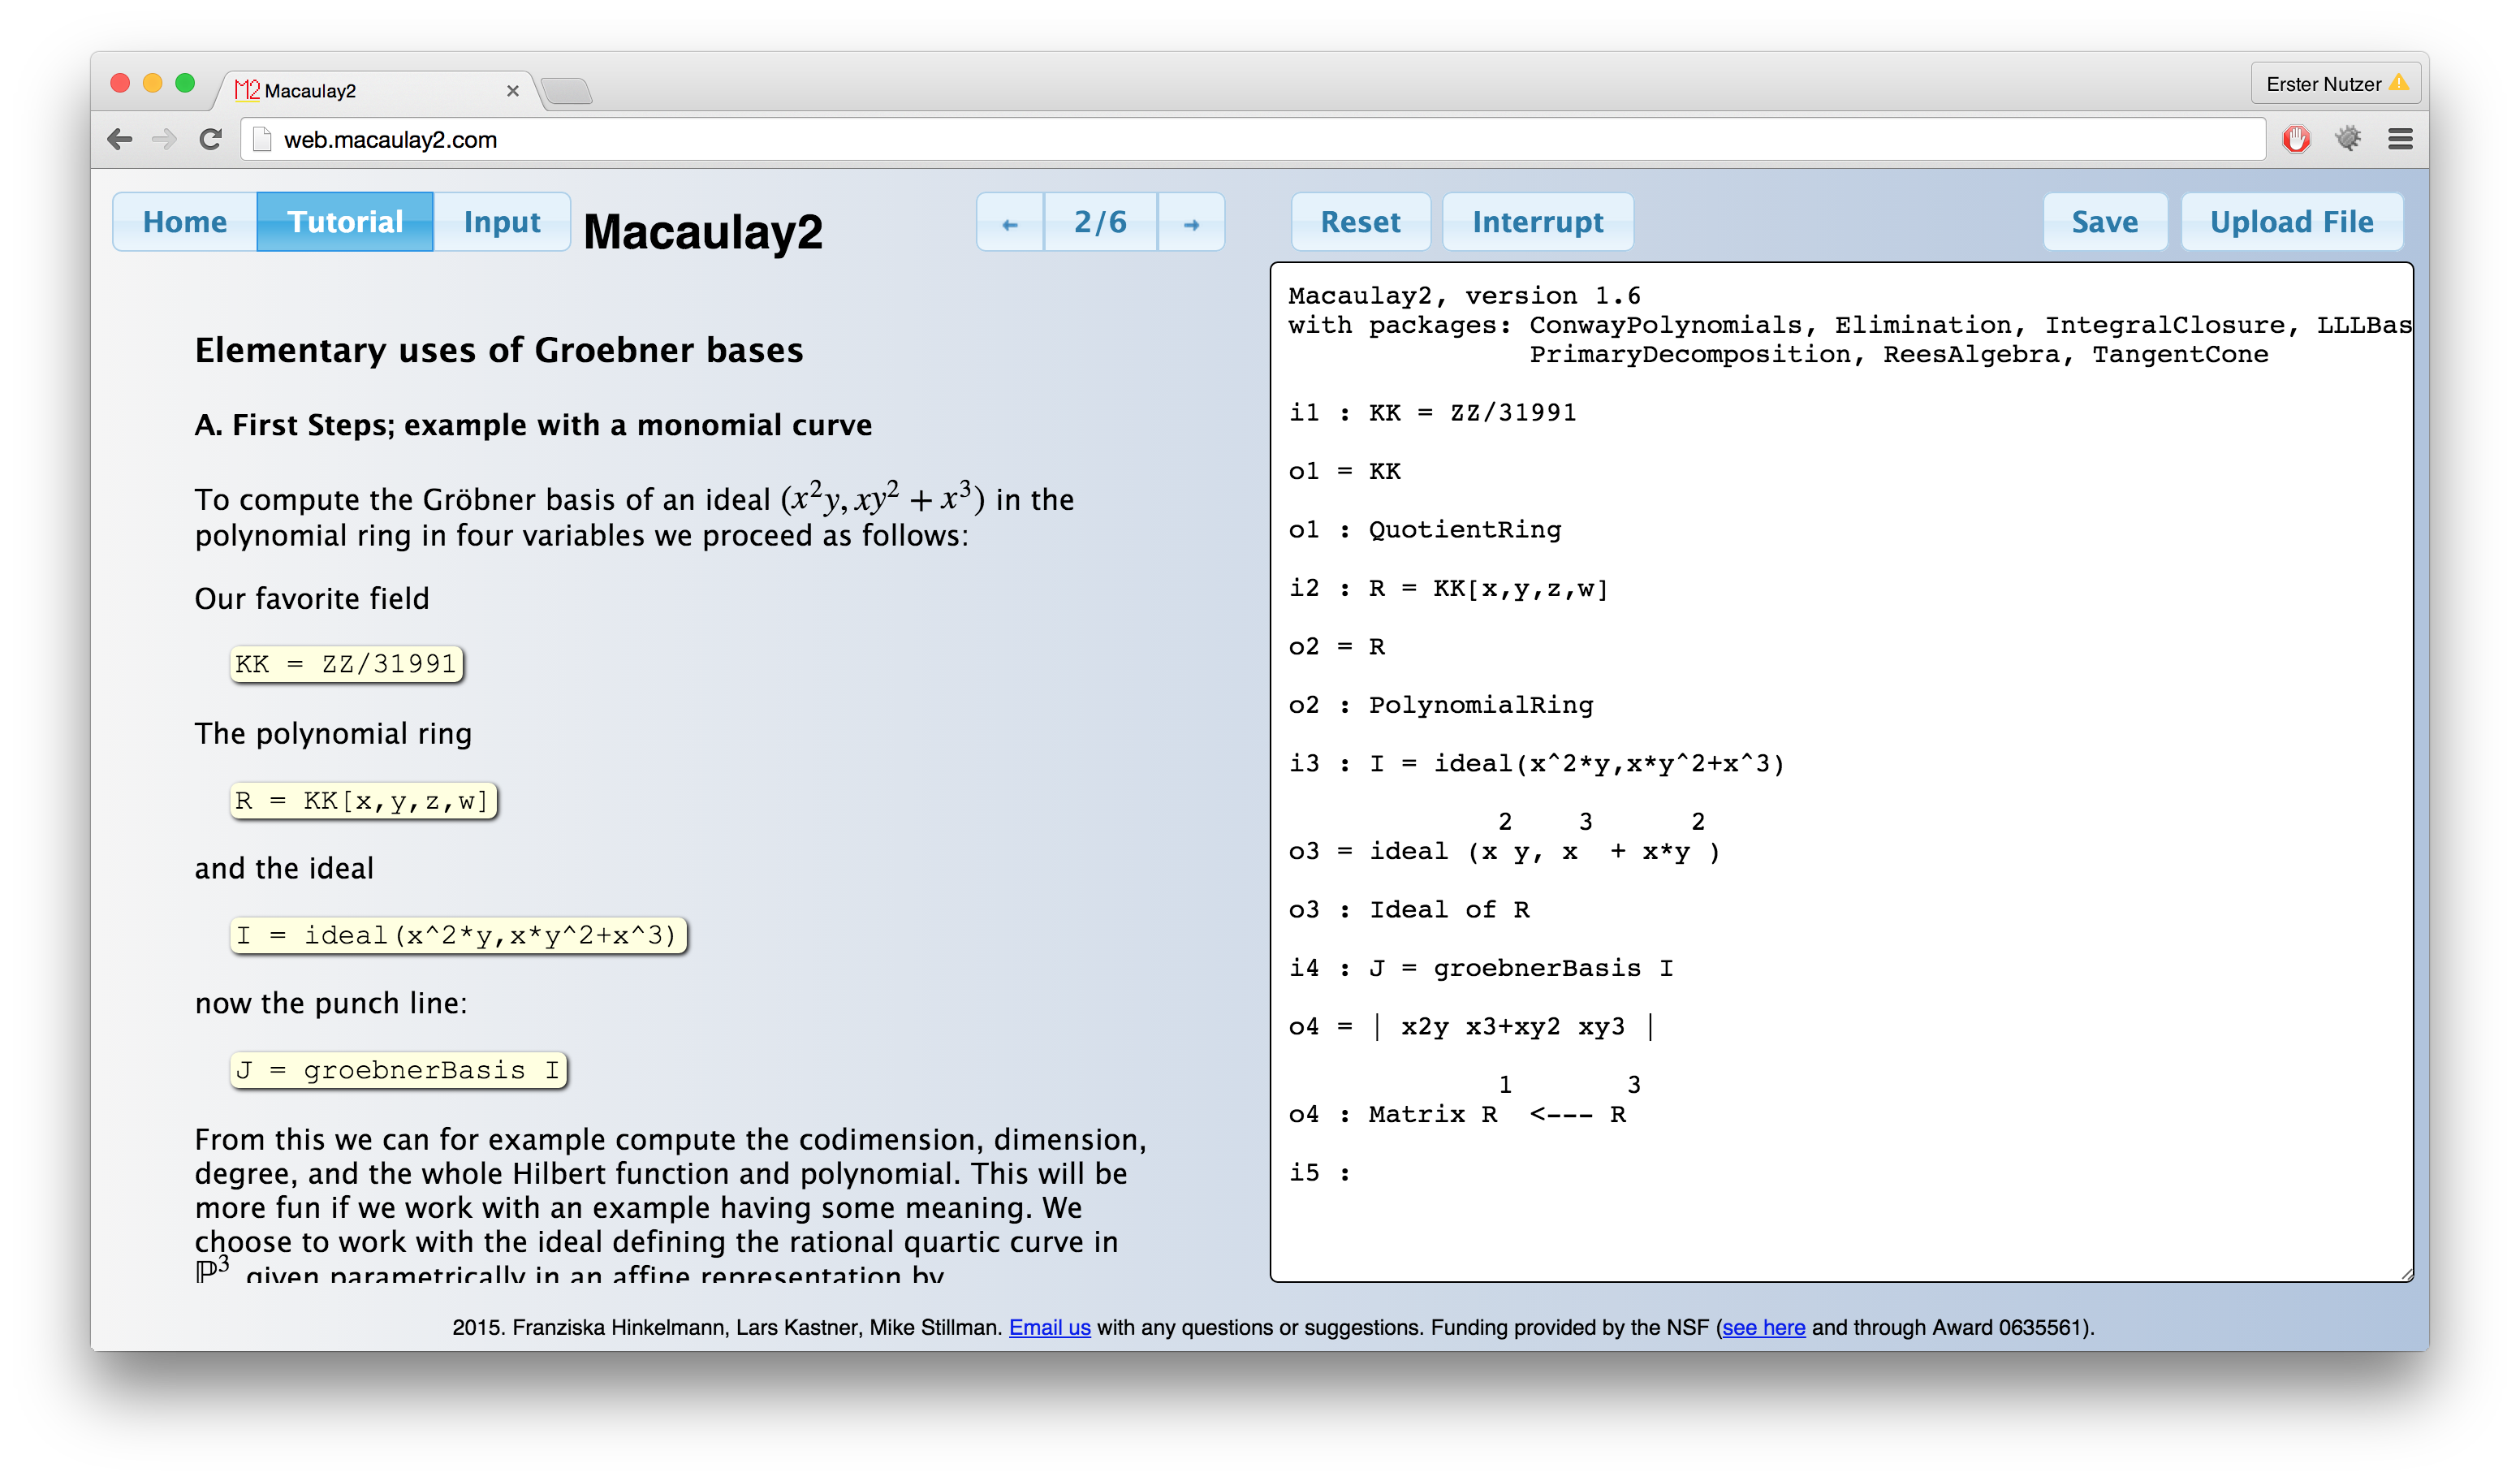
\includegraphics[width=.99\textwidth]{homeWebsite.jpg}
    \caption{A typical view in the web version of \M2. The left hand
        side shows a tutorial giving an introduction to Gr\"obner
        bases. Text in yellow can be clicked and is then executed by
        Macaulay2 on the server. The complete output of the calculations
        is show on the right hand side. Clicking {\it Home, Tutorial, Input}
        changes the left hand view, {\it Reset, Interrupt}
        reset and interrupt the Macaulay2 session on the server, {\it
        Save} provides both the input and the output of the current
        session to the user as a text file, and {\it Upload} uploads files
        that can then be accessed by \M2.}
\label{fig:home}
\end{figure*}



Macaulay2 is a software system devoted to supporting research
in algebraic geometry and commutative algebra, whose creation and
development have been funded by the National Science Foundation
since 1992. We developed a web version of \M2 \cite{M2}. It is available at \cite{webM2}.
The web version has the advantage that users do not need to
download or install any software. A browser and internet connection are enough to
run calculations in \M2. It
has the same functionality as the desktop version,
albeit users might have access to less resources
than on their own machine. Users can upload files,
load packages, and generate files such as images.

Our primary motivation for creating this web application was to
provide an easy to use experience for classroom and student use.
Having students download and install software such as \M2 is time
consuming and inevitably there are some situations for which this
process fails or takes significant effort to get runnning, e.g., on
some versions of Windows.  The web application is designed to
be able to handle many students at once. To keep it as simple as possible,
there is no signup or login process.


 The web version was used at the Syzygyies
meeting in Berlin in May 2013, with about 70 users. It is being used in courses at Cornell
University, Harvard University, Georgia Tech, and Free University of
 Berlin. We would like to point out that the
site is suited not only for beginners, but also for seasoned experts.

We considered off the shelf solutions, such as the Sage
notebook~\cite{sagenotebook}, but decided that we wished for a
lighter-weight solution, and one that did not require users to create
new accounts at a web site.  Nothing available seemed to meet our
needs, hence the current system.

The web version runs under the Chrome, Firefox and Safari web browsers, but not
under Internet Explorer.  On the iPad, it runs under Chrome and
Safari, although it seems that Chrome offers a nicer user experience.
It runs under recent versions of Android ($4.0$ and higher).

In addition to presenting an interface to an instance of \M2
running on a distant server, a number of tutorials to
learn \M2 are provided.  Instructors can create their own
tutorials, and can make them available to their students, as well as
to other \M2 users.  

In Section 2, we describe the basics of using the web application.
Section 3 details how to create and make available your own tutorials.
Providing a program such as \M2 which allows users to
access system resources presents a number of challenges to keep users
from naively or mischievously misusing the system.  In Section 4, we
provide details as to how we structure the application on the server.
In the last section, we describe some of our wish-list items for
improving and extending the system.

The system is open source, and available on github (see \cite{github}).
If you would like more information on using this in your own courses,
or if you have suggestions, please contact one of us.

We would like to thank Charles Boyd, Dan Grayson, Greg Smith, and Benjamin Lorenz for
fruitful discussions on system security and on user interface design.

\section{How to use the website}

An important
design decision is to keep the interface as simple as possible.
Therefore there is no login or registration.

The right hand side provides a shell like environment running
Macaulay2. You can type into it, as well as use the arrow keys for
navigating through your command history.

On the left hand side, the user can navigate between {\it Home}, {\it
  Tutorial}, and {\it Input}. {\it Home} shows the table of contents
of tutorials. {\it Tutorial} shows the currently selected
tutorial. Tutorials are interactive and contain executable pieces of
Macaulay2 code that are run by clicking on them. {\it Input} shows a
terminal window in which the user can type {\it Macaulay2} commands and execute them.

All code executed, either by clicking on interactive parts in a
tutorial or by entering code in the {\it Input} window, appears on the
right hand side together with the output from Macaulay2 to those
results.

The {\it Reset} button resets a Macaulay2 session, i.e., restarts 
the \M2 process: it stops any running calculation, deletes all variables, 
unloads all packages, and then reloads the standard packages.

The {\it Interrupt} button stops a running calculation, without
resetting the Macaulay2 session.

\subsection{Features}

The user is free to run all \M2 commands that are available in the
running version. To find the version of \M2 running on the server,
enter and evaluate: {\tt version\#"VERSION"}.  Loading packages is
done using {\tt loadPackage} or {\tt needsPackage}, e.g. {\tt needsPackage "BoijSoederberg"}.  
New packages can be
uploaded to the user's session, by clicking the {\it Upload file}
button. Similarly, any other file, such as text files, that one might
want to manipulate or read data from with \M2, can be uploaded to
the user's session.

%Loading packages is possible, too, with commands
%such as {\tt loadPackage}. If packages are not available, they can be
%uploaded to the users session, by clicking the {\it Upload file}
%%nbutton. Similarly, any other file, such as text files, that one might
%want to manipulate or read data from with Macaulay2 can be uploaded to
%the user's session.

\begin{figure*}[htb]
    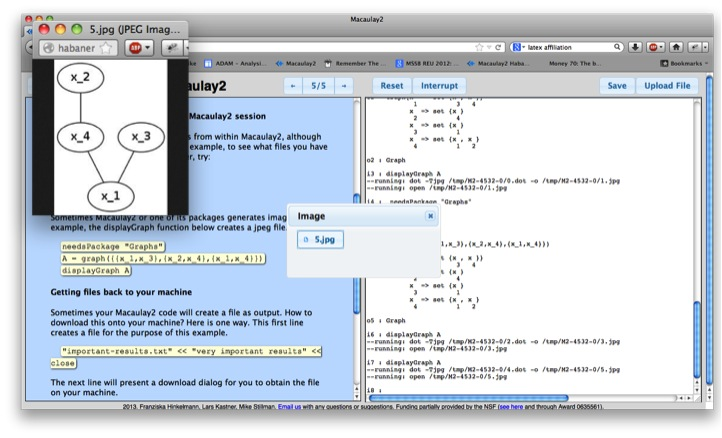
\includegraphics[width=.95\textwidth]{withGraph.jpg}
    \caption{Screenshot after the user
      generated an image. Some Macaulay2 packages can generate
      graphs. By invoking the command {\tt displayGraph}, the image is
      generated on the server and displayed to the user.}
    \label{fig:graph}
\end{figure*}

Results from a session can be retrieved by using the {\it Save}
button, or by using copy and paste. If Macaulay2 generates
images such as graphs, those are presented to the user, see Figure \ref{fig:graph}.

%If the user needs to retrieve
%files that are stored in his session, those can be retrieved by
%executing {\tt open} in the user's session. 

Session are usually kept alive for several days, which allows users to
continue their work next time they access the server, if either they
have not closed their browser, or set the browser to remember their
windows.

\section{Tutorials}

You can create your own tutorials for the web version. If you teach a course,
email your tutorial to your students. They can click
{\it Load Tutorial} on the website and work through the tutorial.
If you want to share tutorial with the community, we would
be happy to include them on the website!

We provide the \M2 package {\it DocConverter}.
It converts a file from {\it SimpleDoc} to the tutorial specific HTML. Please see the
{\it DocConverter} package for instructions and examples.


\section{Internal structure}

We choose to implement the server in Node.js
because of Node.js's event-driven, non-blocking I/O model \cite{nodejs}.
The Node.js server functions as a bridge between Macaulay2 instances and end user.

For every user we start a new Macaulay2 process and
provide them with the underlying linux system in a separate virtual environment.
This allows advanced users to
interact with the file system or run shell commands by using Macaulay2's {\tt get} command.

\begin{lstlisting}[breaklines]
-- get information on the underlying operating system
i8 : get "!uname -ar "
o8 = Linux 35d4e91d4779 3.13.0-48-generic #80-Ubuntu SMP Thu Mar 12 11:16:15 UTC 2015 x86_64 x86_64
     x86_64 GNU/Linux
-- write to a file     
i9 : "important-results.txt" << "very important results" << close
o9 = important-results.txt
o9 : File
-- list all files in the current directory
i21 : get "!ls -l"
o21 = total 4 -rw-r--r-- 1 m2user m2user 22 Apr 12 22:37 important-results.txt
-- obtain the file
i22 : get "!open important-results.txt"
\end{lstlisting}

Technically, this is achieved by using Docker containers \cite{docker}. Docker implements
a high-level API to provide lightweight containers that run processes in isolation.
We start a new Docker container running Macaulay2 for every user. The Node.js
server communicates with Docker containers via {\it ssh}. This allows us to easily
scale the application as demand grows.

To ease the setup process we provide a virtual machine that contains both the Node.js server
and Docker. This virtual machine is configured using {\tt vagrant}, a tool to create and
configure lightweight, reproducible, and portable development environments \cite{vagrant}.

\section{The future}

We envision some form of session sharing which would turn the web app into a tool for collaborative research.

We are collaborating with several mathematicians to develop more tutorials.
We plan to substantically increase the number of tutorials in the tutorial database over the next semester.

The web app was designed with \M2 in mind, but
the entire structure will work for other command line programs such as Singular \cite{singular},
and GAP \cite{GAP4}. A similar web app for Singular is work in progress.


\bibliographystyle{plain}
\bibliography{references}
\end{document}
